\section{Experiments}
We evaluate our method with state-of-the-art wild domain adaptation methods and deep domain adaptation methods using these datasets; Office-31 and Office-Home.
\subsection{Datasets}
\label{sec:datasets}
\textbf{Office-31} \cite{office31} is a popular benchmark domain adaptation dataset consisting of $4652$ images of $31$ categories collected from three domains: Amazon (\textbf{A}), Webcam (\textbf{W}), and DSLR (\textbf{D}). With $3$ domains, $6$ transfer tasks are obtained.\\
\textbf{Office-Home} \cite{officehome} has been created to evaluate domain adaptation algorithms for object recognition using deep learning. It is a more challenging
dataset for visual domain adaptation, consisting of 15,500 images from 65 classes in 4 domains: Artistic images (\textbf{Ar}), Clip Art (\textbf{Cl}), Product images (\textbf{Pr}) and Real-World images (\textbf{Re}). For each domain, the dataset contains images of 65 object categories found typically in Office and Home settings. With $4$ domains, $12$ transfer tasks are obtained.\\

Since both the above datasets are clean, following \cite{e43c87956bec4495a9f947cef8ea2780}, we need to corrupt these datasets manually by the noise transition matrix $M$, where $M_{ij} = Pr(\tilde{y} = j|y = i)$ given that noisy $\tilde{y}$ is flipped from clean $y$. Assume that the matrix $M$ has two representative structures: (1) Symmetry flipping \cite{10.5555/2969239.2969241};
(2) Pair flipping: a simulation of fine-grained classification with noisy labels, where labelers may make mistakes only within very similar classes.\\
\begin{figure}[ht]
            \centering
            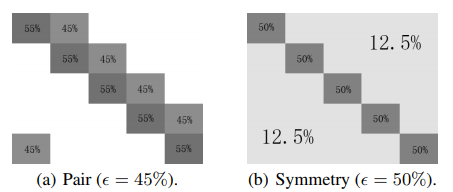
\includegraphics[scale = 0.5]{noise.png}
            \caption{Transition matrices of different noise types.}
\label{fig:noise}
\end{figure}\\
\textbf{Bing-Caltech} \cite{bing-caltech} was created with Bing and Caltech-256 datasets. The Bing dataset was formed by collecting images retrieved by Bing image search for each of the Caltech-256 category labels. Apart from the statistical differences between Bing images and Caltech images, the Bing dataset consists of rich noises, with presence of multiple objects in the same image, polysemy and caricaturization. We simply use Bing as the noisy source domain and Caltech-256 as the clean target domain. While the experiments on Office-31 and Office-Home are random noisy
data, the experiments here represent the performance in real-world weakly-supervised domain adaptation.
\subsection{Baselines}
\label{subsec:baseline}
Our approach can be used as plug in for any standard adversarial domain adaptation network. Here we use DANN\cite{dann} employed with entropy minimization on target data as a backbone. We compare our results with DANN to see how much our approach is able to improve over it. We also compare with TCL \cite{tcl} which is one of the state of the art method for WUDA. We defined two very naive variants of our approach : (1) CT-DANN-1 and (2) CT-DANN-2. In CT-DANN-1, instead of using weighting defined in \ref{eq:weight} we just use small loss samples as in standard co-teaching framework. We must know the noise level for CT-DANN-1 as it is the case in co-teaching too. This is a big disadvantage of this approach. In CT-DANN-2, we first train Network 1 and 2 defined in Figure \ref{fig:networks} using co-teaching framework defined in Algorithm \ref{algo:coteaching}; then only small loss source instances are used to train the DANN network. CT-DANN-2 approach is not end to end approach, however in deep learning world we like to have end to end architectures.
\subsection{Network Set-up and Optimizer}
All deep methods are implemented based on PyTorch. We use ResNet-50 pre-trained on the ImageNet dataset \cite{imagenet} as our base model, and add a fully connected bottleneck layer before its classifier layer. We fine-tune only the last residual block of the ResNet-50 model, and train the bottleneck layer, the classifier layer and the domain discriminator from scratch. The tradeoff hyper-parameter $k$ in equation \ref{eq:weight} is selected according to magnitudes of the two terms and the thresholds $(lower$ , $upper)$ in equation \ref{eq:weight} is selected according to the distribution of classifier probability values on source data i.e. $(G_{y}(G_{f}(x))$. Upper threshold is set close to 0.6 and lower threshold is set close to 0.2. Tradeoff parameters $\lambda_1$ and $\lambda_2$ defined in step 11 of Algorithm \ref{algo: ctdann} are set to be 1 and 0.1. We used mini-batch SGD with momentum of 0.9 and the same learning rate strategy as in \cite{dann}. Gradient reversal layer $(grl)$ is used in the same way as used in the DANN \cite{dann}.
\subsection{Results}
We created 3 label noise vector for source domain data for a particular noise level and noise type (Symmetric or Pairflip) while experimenting with Office 31 and Office-Home. We run all the approaches with label noise vectors generated to have fair comparison among approaches and report the average of the results on 3 label noise vectors for a particular approach. As Bing-Caltech dataset has native noise, so we take it as it is. We did extensive evaluation on Office 31 dataset with noise levels of 40\%, 30\% and 10\%. We expect our approach CT-DANN to perform better over standard domain adaptation in case of high noise and perform almost same in case of low level noise. Experiments with 10\% level noise shows that in the case of low level noise our approach performs similarly in comparison to standard DANN. For Office-Home, we experimented with only 40\% noise. We expect the improvement on Office-Home to be in sync with improvement on Office 31.\\
Table \ref{tab:office_sym} and Table \ref{tab:office_pair} enlists the results of our approach CT-DANN in comparison with DANN and TCL on transfer tasks obtained from Office 31 dataset. It is evident that CT-DANN improves over the backbone DANN much significantly and beating the current state of the art TCL too. In case of low noise i.e. 10\%, performance of CT-DANN approach is close to DANN and TCL which is expected. 

\begin{center}
\begin{table*}[h!]
    \centering
    \begin{tabular}{|c|c|c|c|c|c|c|c|}
    \hline
    \multirow{2}{3em}{Noise Level} & \multirow{2}{4em}{Approach} &  \multicolumn{6}{|c|}{Office 31}\\
    \cline{3-8}
    & & A->D & A->W & D->A & D->W & W->A & W->D\\
    \hline
    \multirow{3}{3em}{10\%} & DANN & 87.05 & 90.94 & 69.72 & 95.58 & 67.09 & 97.42 \\
    & TCL & 88.49 & 91.10 & 67.41 & 96.54 & 67.07 & 98.33\\
    & CT-DANN & 86.50 & 92.12 & 69.73 & 98.09 & 69.50 & 99.78\\
    \hline
    \multirow{3}{3em}{30\%} & DANN & 82.26 & 83.81 & 61.42 & 82.17 & 64.27 & 87.15 \\
    & TCL & 84.56 & 88.73 & 61.42 & 82.82 & 67.15 & 92.59\\
    & CT-DANN & 87.47 & 90.18 & 64.11 & 90.66 & 69.46 & 96.94\\
    \hline
    \multirow{3}{3em}{40\%} & DANN & 73.88 & 78.99 & 60.24 & 76.17 & 54.92 & 76.79 \\
    & TCL & 86.48 & 89.35 & 60.17 & 82.29 & 56.60 & 89.79\\
    & CT-DANN & 84.47 & 90.32 & 63.80 & 86.02 & 64.58 & 92.80\\
    \hline
    \end{tabular}
    \caption{Classification Accuracy (\%) on \textbf{Office-31} with different Symmetric noise levels}
    \label{tab:office_sym}
    \end{table*}
\end{center}

\begin{center}
\begin{table*}[h!]
    \centering
    \begin{tabular}{|c|c|c|c|c|c|c|c|}
    \hline
    \multirow{2}{3em}{Noise Level} & \multirow{2}{4em}{Approach} &  \multicolumn{6}{|c|}{Office 31}\\
    \cline{3-8}
    & & A->D & A->W & D->A & D->W & W->A & W->D\\
    \hline
    
    \multirow{3}{3em}{10\%} & DANN & 00.00 & 00.00 & 00.00 & 00.00 & 00.00 & 00.00 \\
    & TCL & 00.00 & 00.00 & 00.00 & 00.00 & 00.00 & 00.00 \\
    & CT-DANN & 00.00 & 00.00 & 00.00 & 00.00 & 00.00 & 00.00 \\
    \hline
    
    \multirow{3}{3em}{30\%} & DANN & 00.00 & 00.00 & 00.00 & 00.00 & 00.00 & 00.00 \\
    & TCL & 00.00 & 00.00 & 00.00 & 00.00 & 00.00 & 00.00 \\
    & CT-DANN & 00.00 & 00.00 & 00.00 & 00.00 & 00.00 & 00.00 \\
    \hline
    
    \multirow{3}{3em}{40\%} & DANN & 00.00 & 00.00 & 00.00 & 00.00 & 00.00 & 00.00 \\
    & TCL & 00.00 & 00.00 & 00.00 & 00.00 & 00.00 & 00.00 \\
    & CT-DANN & 00.00 & 00.00 & 00.00 & 00.00 & 00.00 & 00.00 \\
    \hline
    \end{tabular}
    \caption{Classification Accuracy (\%) on \textbf{Office-31} with different Pairflip noise levels}
    \label{tab:office_pair}
    \end{table*}

\end{center}

\vspace{-1.4cm}
\begin{center}
\begin{table*}[h!]
    \centering
    \begin{tabular}{|c|c|c|c|c|c|c|c|}
    \hline
    \multirow{2}{3em}{Noise Level} & \multirow{2}{4em}{Approach} &  \multicolumn{6}{|c|}{Office 31}\\
    \cline{3-8}
    & & A->D & A->W & D->A & D->W & W->A & W->D\\
    \hline
    
    \multirow{5}{3em}{40\%} & DANN & 73.88 & 78.99 & 60.24 & 76.17 & 54.92 & 76.79 \\
    & TCL & 86.48 & 89.35 & 60.17 & 82.29 & 56.60 & 89.79\\
    & CT-DANN & 84.47 & 90.32 & 63.80 & 86.02 & 64.58 & 92.80\\
    & CT-DANN-1 & 83.85 & 90.36 & 61.67 & 85.20 & 62.55 & 90.23 \\
    & CT-DANN-2 & 81.63 & 87.08 & 59.96 & 83.72 & 64.54 & 83.98 \\
    \hline
    \end{tabular}
    \caption{Comparison with variants of CT-DANN for 0.4 Symmetric noise level}
    \label{tab:office_var}
    \end{table*}
\end{center}
\vspace{-1cm}
\begin{center}
\begin{table*}[h!]
    \centering
    \resizebox{\columnwidth}{!} & DANN & 00.00 & 00.00 & 00.00 & 00.00 & 00.00 & 00.00 & 00.00 & 00.00 & 00.00 & 00.00 & 00.00 & 00.00 \\
    & TCL & 00.00 & 00.00 & 00.00 & 00.00 & 00.00 & 00.00 & 00.00 & 00.00 & 00.00 & 00.00 & 00.00 & 00.00 \\
    & CT-DANN & 00.00 & 00.00 & 00.00 & 00.00 & 00.00 & 00.00 & 00.00 & 00.00 & 00.00 & 00.00 & 00.00 & 00.00 \\
    \hline
    \end{tabular}
    }
    \caption{Classification Accuracy (\%) on \textbf{Office-Home} with 40\% Symmetric noise levels}
    \end{table*}
\end{center}

\begin{center}
\begin{table*}[h]
    \centering
    \resizebox{\columnwidth}{!} & DANN & 00.00 & 00.00 & 00.00 & 00.00 & 00.00 & 00.00 & 00.00 & 00.00 & 00.00 & 00.00 & 00.00 & 00.00 \\
    & TCL & 00.00 & 00.00 & 00.00 & 00.00 & 00.00 & 00.00 & 00.00 & 00.00 & 00.00 & 00.00 & 00.00 & 00.00 \\
    & CT-DANN & 00.00 & 00.00 & 00.00 & 00.00 & 00.00 & 00.00 & 00.00 & 00.00 & 00.00 & 00.00 & 00.00 & 00.00 \\
    \hline
    \end{tabular}
    }
    \caption{Classification Accuracy (\%) on \textbf{Office-Home} with 40\% Pairflip noise levels}
    \end{table*}
\end{center}
\vspace{-1.2cm}
Table \ref{tab:office_var} lists the results of CT-DANN and its variants (defined in \ref{subsec:baseline}) in comparison with DANN and TCL for 40\% noise level. Performance of CT-DANN-1 is close to CT-DANN, but there is hard assumption of knowing the noise level for CT-DANN-1. With CT-DANN-2, we were able to get improvement over backbone DANN, but it is not an end to end deep architecture and hard assumption of knowing the noise level holds in this also.\\
For Office-Home, we experimented only with 40\% noise Symmetric as well as Pairflip. We expect our approach to perform similarly for other noise level too as that of Office-31.



% \color{red}
% 1. Mean with std for all 4 vectors should be sufficient rather than listing all separately.
% 2. Pairflip and symmetric noise show separately. 
% 10, 20, 30, 40, 50 percent noise - both cases 
% 3. Analysis 
% (a) No noise case - does it degrade performance?
% (b) Sequential - to show integrated algo works
% (c) Without one/both weighting - to show both weighting helps.
% (d) What is the result if we know the noise label vs. we use the proposed weighting strategy.
% Some examples of initial wrong labels and examples of small loss samples.
% - Can we compare with other approaches (maybe more recent) which they have reported?
% - Real dataset - could not find any other dataset other than Bing.
% - Another backbone.
% \color{black}


